\section{Appendix}

\label{sec:appendix}

%%%%%%%%%%%%%%%%%%%%%%%%%%%%%%%%%%%%%%%%%%%%%%%%%%%%%%%

\subsection{One-shot hit-and-run algorithm to draw internal weights for random feature maps}
\label{sec:app:algo:hr}

\begin{algorithm}[!htp]
\caption{Hit-and-run sampling for a row of the internal augmented matrix $\bb{W}_{\rm in}|\bb{b}_{\rm in}$}
\label{algo:hr}
\begin{algorithmic}[1]
\STATE Input: training data $\bb{U}=[\bb{u_1}, \bb{u}_2, \cdots, \bb{u}_N]$. Borders for the good range of the $\tanh$-function $L_{0,1}$. Here $L_0=0.4$ and $L_1=3.5$.
\STATE Sample $b$ uniformly from $(L_0, L_1)$, the "good" part of the domain of $\tanh$.
\STATE Select a sign vector $\bb{s}$ uniformly randomly from $\{-1, 1\}^D$.
\FOR{$i = 1,\cdots,D$}
    \IF{$\bb{s}_i = 1$}
        \STATE $\bb{x}_{-,i} \leftarrow \underset{1\le n\le N}{\min} \bb{u}_{n,i}$
        \STATE $\bb{x}_{+,i} \leftarrow \underset{1\le n\le N}{\max} \bb{u}_{n,i}$
    \ELSE
        \STATE $\bb{x}_{-,i} \leftarrow \underset{1\le n\le N}{\max} \bb{u}_{n,i}$
        \STATE $\bb{x}_{+,i} \leftarrow \underset{1\le n\le N}{\min} \bb{u}_{n,i}$
    \ENDIF
\ENDFOR
\STATE $V\leftarrow\{\bb{w}\in\mathbb{R}^D:\sgn(\mathbf{w}_i)\in\{\mathbf{s}_i, 0\}\;\;\forall\;i=1,2,\ldots,D\}$
\STATE Randomly select a unit vector $\bb{d}\in V$. 
    \STATE $c_0\leftarrow0$.
    \STATE $c_1\leftarrow\inf\left(\left\{\frac{L_0-b}{\bb{d}\cdot \bb{x}_-},\frac{L_1-b}{\bb{d}\cdot \bb{x}_+}\right\}\cap(\mathbb R_{>0}\cup\{+\infty\})\right)$ with the convention $\inf\varnothing=+\infty$.
    \STATE Sample $c$ uniformly from $(c_0, c_1)$.
    \STATE $\bb{w}\leftarrow c\bb{d}$
\STATE Uniformly sample a scalar $z$ from $\{-1, 1\}$.
\IF{$z=1$}
    \STATE $(\bb{w},b)$ is our final row sample. 
\ELSE
    \STATE $-(\bb{w},b)$ is our final row sample. 
\ENDIF
\end{algorithmic}
\end{algorithm}

%%%%%%%%%%%%%%%%%%%%%%%%%%%%%%%%%%%%%%%%%%%%%%%%%%%%%%%

\subsection{Additional numerical details}
\label{ssec:detail}

In this section we document additional numerical details across $5$ tables corresponding to the experimental results in Section~\ref{sec:results}. Each row summarizes the results for $500$ samples that differ in their training data, testing data, and the non-trainable random weights and biases of the corresponding model. Along with the model details and mean, standard deviation, median, minimum and maximum of VPT, each row also shows the corresponding $\beta$ used in the experiments and the average training time in seconds which includes the run-time of algorithm~\ref{algo:hr}. For all models trained on noisy data, a zero-mean Gaussian noise with standard deviation $10^{-3}$ was used. For each architecture, the best performing model has been highlighted with coloring.

%%%%%%%%%%%%%%%%%%%%%%%%%%%%%%%%%%%%%%%%%%%%%%%%%%%%%%%

\subsubsection{Lorenz-63}
\label{ssec:ap-L63} 

We use two different setups for L63. Table~\ref{tab:L63_1_s} documents results for $(N, \Delta t, \varepsilon) = (5\times10^4, 0.01, 0.3)$. This setup also appears in \cite{platt2022systematic}. Table~\ref{tab:L63_0_s} documents results for $(N, \Delta t, \varepsilon) = (2\times10^4, 0.02, \sqrt{0.05})$. This setup also appears in \cite{gottwald2021supervised, mandal2024choice}. A similar setup with $\varepsilon=0.4$ appears in \cite{akiyama2022computational}. To generate the training and testing data for L63 we use a burn-in period of $40$ model time units. $\Lambda_1$ for L63 is $0.91$.


\begin{table}[!htp]
    \centering
    \begin{tabular}{|c|c|c|c|c|c|c|c|c|c|c|} \hline
\multicolumn{4}{|c|}{Model} &\multicolumn{5}{c|}{VPT} & \multicolumn{2}{c|}{}\\ \hline
architecture & $D_r$ & $B$ & model size & mean & std & median & min & max &$\beta$ & $\mathbb{E}[t_{\rm train}]$(s)\\ \hline\hline
\multirow{6}{*}{RFM} & \cellcolor{pink}512 & \cellcolor{pink}1 & \cellcolor{pink}3584 & \cellcolor{pink}9.8 & \cellcolor{pink}1.8 & \cellcolor{pink}9.8 & \cellcolor{pink}4.0 & \cellcolor{pink}16.0 & \cellcolor{pink}3.52e-09 & \cellcolor{pink}1.1e-02\\ \cline{2-11}
 & 1024 & 1 & 7168 & 9.8 & 1.5 & 9.8 & 4.9 & 15.5 & 6.40e-09 & 1.6e-02\\ \cline{2-11}
 & 2048 & 1 & 14336 & 9.3 & 1.5 & 9.3 & 4.0 & 15.3 & 4.96e-08 & 4.4e-02\\ \cline{2-11}
 & 4096 & 1 & 28672 & 9.3 & 1.5 & 9.3 & 3.8 & 13.8 & 8.20e-08 & 1.2e-01\\ \cline{2-11}
 & 8192 & 1 & 57344 & 9.5 & 1.7 & 9.5 & 3.8 & 16.3 & 6.76e-08 & 4.4e-01\\ \cline{2-11}
 & 16384 & 1 & 114688 & 9.5 & 1.5 & 9.6 & 4.9 & 18.9 & 8.92e-08 & 2.1e+00\\ \cline{2-11}
\hline\hline
\multirow{6}{*}{SkipRFM} & 512 & 1 & 3584 & 10.1 & 1.7 & 10.0 & 4.1 & 16.9 & 3.88e-09 & 7.2e-03\\ \cline{2-11}
 & 1024 & 1 & 7168 & 10.5 & 1.5 & 10.5 & 5.5 & 15.1 & 6.40e-09 & 1.6e-02\\ \cline{2-11}
 & 2048 & 1 & 14336 & 10.3 & 1.6 & 10.3 & 5.0 & 19.5 & 3.16e-08 & 4.4e-02\\ \cline{2-11}
 & 4096 & 1 & 28672 & 10.3 & 1.5 & 10.3 & 6.5 & 16.2 & 7.12e-08 & 1.2e-01\\ \cline{2-11}
 & \cellcolor{pink}8192 & \cellcolor{pink}1 & \cellcolor{pink}57344 & \cellcolor{pink}10.6 & \cellcolor{pink}1.5 & \cellcolor{pink}10.7 & \cellcolor{pink}5.2 & \cellcolor{pink}16.1 & \cellcolor{pink}6.76e-08 & \cellcolor{pink}4.4e-01\\ \cline{2-11}
 & 16384 & 1 & 114688 & 10.4 & 1.6 & 10.4 & 5.0 & 17.2 & 2.44e-07 & 2.1e+00\\ \cline{2-11}
\hline\hline
\multirow{19}{*}{DeepSkip} & 1024 & 1 & 10240 & 10.1 & 1.7 & 10.0 & 4.0 & 17.0 & 4.96e-09 & 1.6e-02\\ \cline{2-11}
 & 1024 & 2 & 20480 & 10.9 & 1.7 & 11.0 & 4.9 & 17.7 & 4.96e-09 & 3.2e-02\\ \cline{2-11}
 & 2048 & 1 & 20480 & 7.6 & 1.9 & 7.7 & 0.2 & 13.7 & 8.20e-11 & 4.9e-02\\ \cline{2-11}
 & 1024 & 4 & 40960 & 11.3 & 1.7 & 11.3 & 4.9 & 18.4 & 4.96e-09 & 6.2e-02\\ \cline{2-11}
 & 2048 & 2 & 40960 & 7.6 & 1.8 & 7.7 & 0.2 & 12.8 & 8.20e-11 & 7.5e-02\\ \cline{2-11}
 & 4096 & 1 & 40960 & 9.9 & 1.6 & 9.9 & 3.9 & 18.6 & 5.32e-08 & 1.2e-01\\ \cline{2-11}
 & 1024 & 8 & 81920 & 11.4 & 1.6 & 11.5 & 5.3 & 16.6 & 4.96e-09 & 1.2e-01\\ \cline{2-11}
 & 2048 & 4 & 81920 & 7.2 & 2.0 & 7.3 & 0.3 & 12.2 & 8.20e-11 & 1.5e-01\\ \cline{2-11}
 & 4096 & 2 & 81920 & 10.9 & 1.7 & 11.0 & 4.9 & 19.5 & 5.32e-08 & 2.4e-01\\ \cline{2-11}
 & 8192 & 1 & 81920 & 10.3 & 1.6 & 10.3 & 4.9 & 16.8 & 6.76e-08 & 4.4e-01\\ \cline{2-11}
 & 1024 & 16 & 163840 & 11.7 & 1.7 & 11.8 & 6.3 & 21.2 & 4.96e-09 & 2.4e-01\\ \cline{2-11}
 & 2048 & 8 & 163840 & 7.2 & 1.9 & 7.2 & 0.3 & 13.7 & 8.20e-11 & 3.1e-01\\ \cline{2-11}
 & 4096 & 4 & 163840 & 11.0 & 1.6 & 11.1 & 4.9 & 16.4 & 5.32e-08 & 4.9e-01\\ \cline{2-11}
 & 8192 & 2 & 163840 & 11.0 & 1.5 & 11.1 & 5.0 & 16.0 & 6.76e-08 & 9.0e-01\\ \cline{2-11}
 & 16384 & 1 & 163840 & 10.7 & 1.6 & 10.7 & 5.6 & 17.8 & 8.92e-08 & 2.1e+00\\ \cline{2-11}
 & \cellcolor{pink}1024 & \cellcolor{pink}32 & \cellcolor{pink}327680 & \cellcolor{pink}12.0 & \cellcolor{pink}1.5 & \cellcolor{pink}12.0 & \cellcolor{pink}6.4 & \cellcolor{pink}20.1 & \cellcolor{pink}4.96e-09 & \cellcolor{pink}4.6e-01\\ \cline{2-11}
 & 4096 & 8 & 327680 & 11.2 & 1.6 & 11.3 & 6.3 & 18.4 & 5.32e-08 & 1.0e+00\\ \cline{2-11}
 & 8192 & 4 & 327680 & 11.2 & 1.6 & 11.3 & 5.2 & 18.3 & 6.76e-08 & 1.8e+00\\ \cline{2-11}
 & 16384 & 2 & 327680 & 10.9 & 1.5 & 10.9 & 5.0 & 17.3 & 8.92e-08 & 4.3e+00\\ \cline{2-11}
\cline{1-2}
\end{tabular}
    \caption{Results for L63 with $N=5\times10^4$, $\Delta t=0.01$ and $\varepsilon=0.3$.}
    \label{tab:L63_1_s}
\end{table}

\begin{table}[!htp]
    \centering
    \begin{tabular}{|c|c|c|c|c|c|c|c|c|c|c|} \hline
\multicolumn{4}{|c|}{Model} &\multicolumn{5}{c|}{VPT} & \multicolumn{2}{c|}{}\\ \hline
architecture & $D_r$ & $B$ & model size & mean & std & median & min & max &$\beta$ & $\mathbb{E}[t_{\rm train}]$(s)\\ \hline\hline
\multirow{6}{*}{SkipRFM} & 512 & 1 & 3584 & 10.1 & 1.7 & 10.0 & 4.6 & 16.7 & 6.04e-10 & 8.8e-03\\ \cline{2-11}
 & \cellcolor{pink}1024 & \cellcolor{pink}1 & \cellcolor{pink}7168 & \cellcolor{pink}10.4 & \cellcolor{pink}1.4 & \cellcolor{pink}10.4 & \cellcolor{pink}4.8 & \cellcolor{pink}16.1 & \cellcolor{pink}8.74e-10 & \cellcolor{pink}1.1e-02\\ \cline{2-11}
 & 2048 & 1 & 14336 & 10.0 & 1.5 & 10.1 & 4.7 & 17.5 & 4.24e-09 & 2.6e-02\\ \cline{2-11}
 & 4096 & 1 & 28672 & 10.1 & 1.4 & 10.1 & 4.8 & 15.7 & 9.46e-09 & 6.2e-02\\ \cline{2-11}
 & 8192 & 1 & 57344 & 10.1 & 1.5 & 10.1 & 4.7 & 15.9 & 2.26e-08 & 2.2e-01\\ \cline{2-11}
 & 16384 & 1 & 114688 & 10.3 & 1.5 & 10.2 & 4.7 & 15.9 & 2.62e-08 & 8.9e-01\\ \cline{2-11}
\hline\hline
\multirow{15}{*}{DeepSkip} & 1024 & 1 & 10240 & 9.7 & 1.6 & 9.7 & 4.6 & 16.0 & 9.46e-10 & 1.1e-02\\ \cline{2-11}
 & 1024 & 2 & 20480 & 10.9 & 1.6 & 10.7 & 4.8 & 17.3 & 9.46e-10 & 2.1e-02\\ \cline{2-11}
 & 1024 & 4 & 40960 & 11.0 & 1.6 & 10.8 & 5.6 & 17.7 & 9.46e-10 & 4.2e-02\\ \cline{2-11}
 & 4096 & 1 & 40960 & 9.8 & 1.6 & 9.8 & 4.6 & 16.9 & 9.28e-09 & 6.2e-02\\ \cline{2-11}
 & 1024 & 8 & 81920 & 11.3 & 1.5 & 11.2 & 4.8 & 17.5 & 9.46e-10 & 7.7e-02\\ \cline{2-11}
 & 4096 & 2 & 81920 & 10.6 & 1.5 & 10.6 & 4.7 & 17.1 & 9.28e-09 & 1.3e-01\\ \cline{2-11}
 & 8192 & 1 & 81920 & 9.2 & 1.4 & 9.2 & 4.6 & 14.2 & 3.70e-08 & 2.2e-01\\ \cline{2-11}
 & 1024 & 16 & 163840 & 11.7 & 1.6 & 11.6 & 6.4 & 18.2 & 9.46e-10 & 1.5e-01\\ \cline{2-11}
 & 4096 & 4 & 163840 & 10.8 & 1.6 & 10.7 & 4.8 & 18.2 & 9.28e-09 & 2.5e-01\\ \cline{2-11}
 & 8192 & 2 & 163840 & 10.4 & 1.5 & 10.4 & 5.4 & 17.8 & 3.70e-08 & 4.4e-01\\ \cline{2-11}
 & 16384 & 1 & 163840 & 9.5 & 1.4 & 9.6 & 4.7 & 14.5 & 5.14e-08 & 8.9e-01\\ \cline{2-11}
 & \cellcolor{pink}1024 & \cellcolor{pink}32 & \cellcolor{pink}327680 & \cellcolor{pink}11.8 & \cellcolor{pink}1.5 & \cellcolor{pink}11.7 & \cellcolor{pink}7.8 & \cellcolor{pink}18.2 & \cellcolor{pink}9.46e-10 & \cellcolor{pink}3.1e-01\\ \cline{2-11}
 & 4096 & 8 & 327680 & 11.0 & 1.4 & 11.0 & 5.6 & 18.2 & 9.28e-09 & 5.1e-01\\ \cline{2-11}
 & 8192 & 4 & 327680 & 10.6 & 1.5 & 10.6 & 5.5 & 15.2 & 3.70e-08 & 9.0e-01\\ \cline{2-11}
 & 16384 & 2 & 327680 & 10.5 & 1.5 & 10.5 & 5.5 & 18.2 & 5.14e-08 & 1.8e+00\\ \cline{2-11}
\cline{1-2}
\end{tabular}
    \caption{Results for L63 with $N=2\times10^4$, $\Delta t=0.02$ and $\varepsilon=\sqrt{0.05}\approx0.224$.}
    \label{tab:L63_0_s}
\end{table}

\subsubsection{Lorenz-96}\label{ssec:ap-L96}
For 40-dimensional L96 with forcing $F=10$ we use $(N, \Delta t, \varepsilon) = (10^5, 0.01, \sqrt{0.5})$. This setup also appears in \cite{platt2022systematic, vlachas2020backpropagation}. Tables~\ref{tab:L96_1_s} and \ref{tab:L96_1_s-l}  document the results for non-local and local architectures respectively. Note that \cite{platt2022systematic} uses $F=8$ and \cite{vlachas2020backpropagation} uses both $F=8$ and $10$. Section~4 of \cite{vlachas2020backpropagation} shows that trained surrogate models demonstrate similar forecasting skill for both values of $F$. This justifies comparing our results with \cite{ platt2022systematic, vlachas2020backpropagation}. To generate the training and testing data for L96 we use a burn-in period of $1000$ model time units. $\Lambda_1$ for L96 is $2.27$. The training data for L96 is well-conditioned, so introducing noise does not enhance the quality of the trained surrogate model. For an example, refer to the last row of Table~\ref{tab:L96_1_s-l}.

\begin{table}[!htp]
    \centering
    \begin{tabular}{|c|c|c|c|c|c|c|c|c|c|c|} \hline
\multicolumn{4}{|c|}{Model} &\multicolumn{5}{c|}{VPT} & \multicolumn{2}{c|}{}\\ \hline
architecture & $D_r$ & $B$ & model size & mean & std & median & min & max &$\beta$ & $\mathbb{E}[t_{\rm train}]$(s)\\ \hline\hline
\multirow{5}{*}{SkipRFM} & 512 & 1 & 41472 & 0.3 & 0.1 & 0.3 & 0.2 & 0.7 & 3.52e-09 & 1.6e-02\\ \cline{2-11}
 & 1024 & 1 & 82944 & 1.0 & 0.2 & 0.9 & 0.6 & 2.1 & 6.40e-09 & 2.4e-02\\ \cline{2-11}
 & 2048 & 1 & 165888 & 2.0 & 0.5 & 2.0 & 1.0 & 4.4 & 4.60e-08 & 6.6e-02\\ \cline{2-11}
 & 4096 & 1 & 331776 & 2.2 & 0.5 & 2.2 & 1.1 & 4.1 & 3.16e-07 & 2.3e-01\\ \cline{2-11}
 & \cellcolor{pink}8192 & \cellcolor{pink}1 & \cellcolor{pink}663552 & \cellcolor{pink}2.3 & \cellcolor{pink}0.6 & \cellcolor{pink}2.3 & \cellcolor{pink}1.2 & \cellcolor{pink}4.2 & \cellcolor{pink}3.16e-07 & \cellcolor{pink}1.0e+00\\ \cline{2-11}
\hline\hline
\multirow{5}{*}{DeepSkip} & 4096 & 1 & 495616 & 2.3 & 0.5 & 2.2 & 1.1 & 4.8 & 1.72e-07 & 2.4e-01\\ \cline{2-11}
 & 4096 & 2 & 991232 & 2.7 & 0.6 & 2.6 & 1.1 & 5.0 & 1.72e-07 & 5.0e-01\\ \cline{2-11}
 & 4096 & 4 & 1982464 & 2.7 & 0.6 & 2.7 & 1.4 & 5.0 & 1.72e-07 & 1.0e+00\\ \cline{2-11}
 & 4096 & 8 & 3964928 & 2.8 & 0.6 & 2.8 & 1.5 & 4.6 & 1.72e-07 & 2.0e+00\\ \cline{2-11}
 & \cellcolor{pink}4096 & \cellcolor{pink}16 & \cellcolor{pink}7929856 & \cellcolor{pink}2.8 & \cellcolor{pink}0.6 & \cellcolor{pink}2.8 & \cellcolor{pink}1.5 & \cellcolor{pink}5.7 & \cellcolor{pink}1.72e-07 & \cellcolor{pink}4.0e+00\\ \cline{2-11}
\cline{1-2}
\end{tabular}
\caption{Results for non-local architectures for L96 with $N=10^5$, $\Delta t=0.01$ and $\varepsilon=0.5$.}
    \label{tab:L96_1_s}
\end{table}


\begin{table}[!htp]
    \centering
    \begin{tabular}{|c|c|c|c|c|c|c|c|c|c|c|} \hline
\multicolumn{4}{|c|}{Model} &\multicolumn{5}{c|}{VPT} & \multicolumn{2}{c|}{}\\ \hline
architecture & $D_r$ & $B$ & model size & mean & std & median & min & max &$\beta$ & $\mathbb{E}[t_{\rm train}]$(s)\\ \hline\hline
\multirow{6}{*}{LocalSkip$_{2,2}$} & 512 & 1 & 6656 & 4.4 & 0.9 & 4.3 & 2.0 & 7.6 & 3.16e-09 & 6.3e-02\\ \cline{2-11}
 & 1024 & 1 & 13312 & 5.3 & 1.1 & 5.3 & 1.9 & 9.1 & 3.16e-08 & 7.8e-02\\ \cline{2-11}
 & 2048 & 1 & 26624 & 5.7 & 1.0 & 5.7 & 3.2 & 8.9 & 8.92e-08 & 1.2e-01\\ \cline{2-11}
 & 4096 & 1 & 53248 & 6.5 & 1.2 & 6.4 & 3.5 & 11.1 & 1.00e-07 & 2.8e-01\\ \cline{2-11}
 & 8192 & 1 & 106496 & 6.7 & 1.1 & 6.8 & 4.1 & 10.4 & 4.24e-07 & 1.1e+00\\ \cline{2-11}
 & \cellcolor{pink}16384 & \cellcolor{pink}1 & \cellcolor{pink}212992 & \cellcolor{pink}6.8 & \cellcolor{pink}1.2 & \cellcolor{pink}6.8 & \cellcolor{pink}3.4 & \cellcolor{pink}10.7 & \cellcolor{pink}7.48e-07 & \cellcolor{pink}4.4e+00\\ \cline{2-11}
\hline\hline
\multirow{9}{*}{LocalDeepRFM$_{2,2}$} & 512 & 4 & 30720 & 4.8 & 0.9 & 4.7 & 2.3 & 7.4 & 5.32e-09 & 4.7e-02\\ \cline{2-11}
 & 1024 & 4 & 61440 & 5.9 & 1.1 & 5.9 & 2.8 & 9.2 & 1.72e-08 & 9.1e-02\\ \cline{2-11}
 & 2048 & 4 & 122880 & 6.2 & 1.1 & 6.2 & 2.9 & 9.5 & 1.36e-07 & 2.7e-01\\ \cline{2-11}
 & 4096 & 4 & 245760 & 6.6 & 1.2 & 6.6 & 3.5 & 10.0 & 1.72e-07 & 9.4e-01\\ \cline{2-11}
 & 8192 & 2 & 245760 & 6.9 & 1.2 & 7.0 & 4.0 & 11.1 & 3.16e-07 & 2.0e+00\\ \cline{2-11}
 & 11586 & 2 & 347580 & 7.1 & 1.3 & 7.0 & 3.9 & 11.5 & 3.52e-07 & 4.3e+00\\ \cline{2-11}
 & 8192 & 4 & 491520 & 7.0 & 1.3 & 7.0 & 3.7 & 11.2 & 3.16e-07 & 4.2e+00\\ \cline{2-11}
 & \cellcolor{pink}16384 & \cellcolor{pink}2 & \cellcolor{pink}491520 & \cellcolor{pink}7.2 & \cellcolor{pink}1.3 & \cellcolor{pink}7.1 & \cellcolor{pink}3.9 & \cellcolor{pink}11.3 & \cellcolor{pink}3.88e-07 & \cellcolor{pink}9.5e+00\\ \cline{2-11}
 & 11586 & 4 & 695160 & 7.1 & 1.3 & 7.0 & 4.0 & 11.2 & 3.52e-07 & 8.8e+00\\ \cline{2-11}
\hline\hline
\multirow{1}{*}{LocalDeepSkip$_{1,4}$} & \cellcolor{pink}16384 & \cellcolor{pink}2 & \cellcolor{pink}393216 & \cellcolor{pink}6.9 & \cellcolor{pink}1.3 & \cellcolor{pink}6.9 & \cellcolor{pink}3.7 & \cellcolor{pink}11.1 & \cellcolor{pink}6.40e-07 & \cellcolor{pink}9.4e+00\\ \cline{2-11}
\hline\hline
\multirow{24}{*}{LocalDeepSkip$_{2,2}$} & 1024 & 1 & 15360 & 5.5 & 1.1 & 5.5 & 2.7 & 8.7 & 9.64e-09 & 9.7e-02\\ \cline{2-11}
 & 1024 & 2 & 30720 & 5.8 & 1.2 & 5.8 & 2.5 & 10.4 & 9.64e-09 & 1.2e-01\\ \cline{2-11}
 & 2048 & 1 & 30720 & 5.8 & 1.1 & 5.7 & 2.3 & 9.2 & 4.96e-08 & 1.3e-01\\ \cline{2-11}
 & 1024 & 4 & 61440 & 6.0 & 1.2 & 5.9 & 2.5 & 9.3 & 9.64e-09 & 1.6e-01\\ \cline{2-11}
 & 2048 & 2 & 61440 & 6.3 & 1.2 & 6.2 & 2.7 & 11.1 & 4.96e-08 & 2.0e-01\\ \cline{2-11}
 & 4096 & 1 & 61440 & 6.0 & 1.1 & 5.9 & 3.5 & 10.0 & 3.88e-07 & 3.2e-01\\ \cline{2-11}
 & 1024 & 8 & 122880 & 6.0 & 1.1 & 6.0 & 2.9 & 9.0 & 9.64e-09 & 2.5e-01\\ \cline{2-11}
 & 2048 & 4 & 122880 & 6.4 & 1.2 & 6.4 & 3.4 & 10.5 & 4.96e-08 & 3.4e-01\\ \cline{2-11}
 & 4096 & 2 & 122880 & 6.6 & 1.2 & 6.6 & 3.0 & 10.1 & 3.88e-07 & 5.8e-01\\ \cline{2-11}
 & 8192 & 1 & 122880 & 6.2 & 1.1 & 6.2 & 3.5 & 9.6 & 9.64e-07 & 1.2e+00\\ \cline{2-11}
 & 1024 & 16 & 245760 & 6.1 & 1.2 & 6.0 & 3.3 & 10.5 & 9.64e-09 & 4.3e-01\\ \cline{2-11}
 & 2048 & 8 & 245760 & 6.5 & 1.2 & 6.5 & 2.6 & 10.2 & 4.96e-08 & 6.1e-01\\ \cline{2-11}
 & 4096 & 4 & 245760 & 6.7 & 1.2 & 6.7 & 3.7 & 10.4 & 3.88e-07 & 1.1e+00\\ \cline{2-11}
 & 8192 & 2 & 245760 & 6.8 & 1.3 & 6.7 & 3.4 & 10.4 & 9.64e-07 & 2.3e+00\\ \cline{2-11}
 & 16384 & 1 & 245760 & 7.0 & 1.2 & 7.0 & 3.9 & 11.1 & 3.88e-07 & 4.5e+00\\ \cline{2-11}
 & 1024 & 32 & 491520 & 6.3 & 1.2 & 6.2 & 3.0 & 10.1 & 9.64e-09 & 7.8e-01\\ \cline{2-11}
 & 2048 & 16 & 491520 & 6.6 & 1.2 & 6.6 & 3.2 & 11.5 & 4.96e-08 & 1.1e+00\\ \cline{2-11}
 & 4096 & 8 & 491520 & 6.9 & 1.2 & 6.8 & 4.1 & 10.7 & 3.88e-07 & 2.1e+00\\ \cline{2-11}
 & 8192 & 4 & 491520 & 7.0 & 1.2 & 6.9 & 3.4 & 12.1 & 9.64e-07 & 4.5e+00\\ \cline{2-11}
 & \cellcolor{pink}16384 & \cellcolor{pink}2 & \cellcolor{pink}491520 & \cellcolor{pink}7.3 & \cellcolor{pink}1.2 & \cellcolor{pink}7.2 & \cellcolor{pink}4.3 & \cellcolor{pink}11.7 & \cellcolor{pink}3.88e-07 & \cellcolor{pink}9.1e+00\\ \cline{2-11}
 & 2048 & 32 & 983040 & 6.7 & 1.2 & 6.7 & 4.1 & 10.8 & 4.96e-08 & 2.2e+00\\ \cline{2-11}
 & 4096 & 16 & 983040 & 7.0 & 1.3 & 7.0 & 3.7 & 11.1 & 3.88e-07 & 4.1e+00\\ \cline{2-11}
 & 8192 & 8 & 983040 & 7.1 & 1.3 & 7.0 & 3.9 & 12.0 & 9.64e-07 & 8.9e+00\\ \cline{2-11}
 & 16384 & 4 & 983040 & 7.2 & 1.2 & 7.2 & 4.1 & 11.8 & 3.88e-07 & 1.8e+01\\ \cline{2-11}
\hline\hline
\multirow{1}{*}{LocalDeepSkipN$_{2,2}$} & \cellcolor{pink}16384 & \cellcolor{pink}2 & \cellcolor{pink}491520 & \cellcolor{pink}7.1 & \cellcolor{pink}1.3 & \cellcolor{pink}7.1 & \cellcolor{pink}3.8 & \cellcolor{pink}10.8 & \cellcolor{pink}3.88e-07 & \cellcolor{pink}9.5e+00\\ \cline{2-11}
\cline{1-2}
\end{tabular}
    \caption{Results for local architectures for L96 with $N=10^5$, $\Delta t=0.01$ and $\varepsilon=0.5$.}
    \label{tab:L96_1_s-l}
\end{table}

%%%%%%%%%%%%%%%%%%%%%%%%%%%%%%%%%%%%%%%%%%%%%%%%%%%%%%%

\subsubsection{Kuramoto-Sivashinsky}
\label{ssec:ap-KS}

For KS with domain length $L=200$ and $512$ spatial grid points we use $(N, \Delta t, \varepsilon) = (10^5, 0.25, 0.5)$. Table~\ref{tab:KS_1} documents the corresponding results. This setup also appears in \cite{vlachas2020backpropagation}. To generate the training and testing data for KS we use a burn-in period of $2.5\times10^4$ model time units. $\Lambda_1$ for KS is $0.094$. We used the following function as our initial condition,
\begin{align}
    \cos\left(\frac{2\pi x}{L}\right)\left(1+\sin\left(\frac{2\pi x}{L}\right)\right).
\end{align}

\begin{table}[!htp]
    \centering
    \begin{tabular}{|c|c|c|c|c|c|c|c|c|c|c|} \hline
\multicolumn{4}{|c|}{Model} &\multicolumn{5}{c|}{VPT} & \multicolumn{2}{c|}{}\\ \hline
architecture & $D_r$ & $B$ & model size & mean & std & median & min & max &$\beta$ & $\mathbb{E}[t_{\rm train}]$(s)\\ \hline\hline
\multirow{2}{*}{LocalRFM$_{8,1}$} & 8192 & 1 & 270336 & 3.6 & 1.3 & 3.9 & 0.5 & 6.5 & 8.56e-06 & 1.2e+00\\ \cline{2-11}
 & \cellcolor{pink}15000 & \cellcolor{pink}1 & \cellcolor{pink}495000 & \cellcolor{pink}4.3 & \cellcolor{pink}0.8 & \cellcolor{pink}4.3 & \cellcolor{pink}1.5 & \cellcolor{pink}6.3 & \cellcolor{pink}2.80e-05 & \cellcolor{pink}4.1e+00\\ \cline{2-11}
\hline\hline
\multirow{6}{*}{LocalDeepRFM$_{8,1}$} & 8192 & 2 & 671744 & 4.0 & 1.3 & 4.2 & 0.5 & 6.8 & 4.60e-06 & 2.1e+00\\ \cline{2-11}
 & 8192 & 3 & 1007616 & 4.5 & 1.0 & 4.6 & 1.0 & 7.1 & 3.52e-05 & 3.1e+00\\ \cline{2-11}
 & \cellcolor{pink}14000 & \cellcolor{pink}2 & \cellcolor{pink}1148000 & \cellcolor{pink}4.8 & \cellcolor{pink}1.0 & \cellcolor{pink}4.9 & \cellcolor{pink}2.1 & \cellcolor{pink}7.1 & \cellcolor{pink}2.00e-05 & \cellcolor{pink}6.5e+00\\ \cline{2-11}
 & 15000 & 2 & 1230000 & 4.6 & 0.9 & 4.7 & 2.1 & 6.9 & 4.24e-05 & 7.4e+00\\ \cline{2-11}
 & 15000 & 3 & 1845000 & 4.7 & 1.0 & 4.8 & 1.7 & 7.3 & 3.88e-05 & 1.1e+01\\ \cline{2-11}
 & 13308 & 5 & 2728140 & 4.6 & 1.0 & 4.7 & 1.9 & 7.0 & 9.55e-05 & 1.5e+01\\ \cline{2-11}
\hline\hline
\multirow{1}{*}{LocalDeepSkip$_{8,1}$} & \cellcolor{pink}15000 & \cellcolor{pink}2 & \cellcolor{pink}1230000 & \cellcolor{pink}0.5 & \cellcolor{pink}0.1 & \cellcolor{pink}0.5 & \cellcolor{pink}0.4 & \cellcolor{pink}0.8 & \cellcolor{pink}2.00e-05 & \cellcolor{pink}7.9e+00\\ \cline{2-11}
\hline\hline
\multirow{1}{*}{LocalRFMN$_{8,1}$} & \cellcolor{pink}15000 & \cellcolor{pink}1 & \cellcolor{pink}495000 & \cellcolor{pink}4.3 & \cellcolor{pink}0.9 & \cellcolor{pink}4.4 & \cellcolor{pink}2.0 & \cellcolor{pink}6.4 & \cellcolor{pink}4.24e-05 & \cellcolor{pink}3.8e+00\\ \cline{2-11}
\hline\hline
\multirow{1}{*}{LocalSkipN$_{8,1}$} & \cellcolor{pink}15000 & \cellcolor{pink}1 & \cellcolor{pink}495000 & \cellcolor{pink}4.3 & \cellcolor{pink}0.8 & \cellcolor{pink}4.4 & \cellcolor{pink}2.0 & \cellcolor{pink}6.4 & \cellcolor{pink}4.24e-05 & \cellcolor{pink}3.8e+00\\ \cline{2-11}
\hline\hline
\multirow{2}{*}{LocalDeepRFMN$_{8,1}$} & 14000 & 2 & 1148000 & 4.9 & 0.9 & 5.1 & 2.7 & 7.0 & 2.00e-05 & 6.3e+00\\ \cline{2-11}
 & \cellcolor{pink}15000 & \cellcolor{pink}2 & \cellcolor{pink}1230000 & \cellcolor{pink}5.0 & \cellcolor{pink}0.9 & \cellcolor{pink}5.0 & \cellcolor{pink}2.7 & \cellcolor{pink}7.6 & \cellcolor{pink}2.00e-05 & \cellcolor{pink}7.6e+00\\ \cline{2-11}
\hline\hline
\multirow{1}{*}{LocalDeepSkipN$_{8,1}$} & \cellcolor{pink}15000 & \cellcolor{pink}2 & \cellcolor{pink}1230000 & \cellcolor{pink}5.0 & \cellcolor{pink}0.9 & \cellcolor{pink}5.1 & \cellcolor{pink}2.6 & \cellcolor{pink}7.7 & \cellcolor{pink}2.00e-05 & \cellcolor{pink}7.9e+00\\ \cline{2-11}
\hline\hline
\end{tabular}
    \caption{Results for KS with $N=10^5$, $\Delta t=0.25$ and $\varepsilon=0.5$.}
    \label{tab:KS_1}
\end{table}

\subsection{Localization schemes}
\label{ssec:loc}

In this section we discuss the efficacy of various localization schemes for L96 and KS. Figures~\ref{fig:L96-loc} and \ref{fig:KS-loc} show crude estimates of expected VPT as a function of $\beta$ for these systems respectively. These estimates were computed by averaging over $5$ samples differing in the training data, the testing data and the non-trainable internal weights and biases for each value of $\beta$. Note that all the data shown in this section correspond to a fixed training data size $N=10^5$. Figure~\ref{fig:L96-loc} shows that $(G, I)=(1, 4)$ and $(2, 2)$ are the best performing localization schemes for L96 and Figure~\ref{fig:KS-loc} shows that overall $(G, I)=(8, 1)$ is the best performing localization scheme for KS. Comparing the first and second panels of Figure~\ref{fig:KS-loc} we see that the optimal localization scheme can be different for different values of $D_r$.

\begin{figure}[!htp]
    \centering
    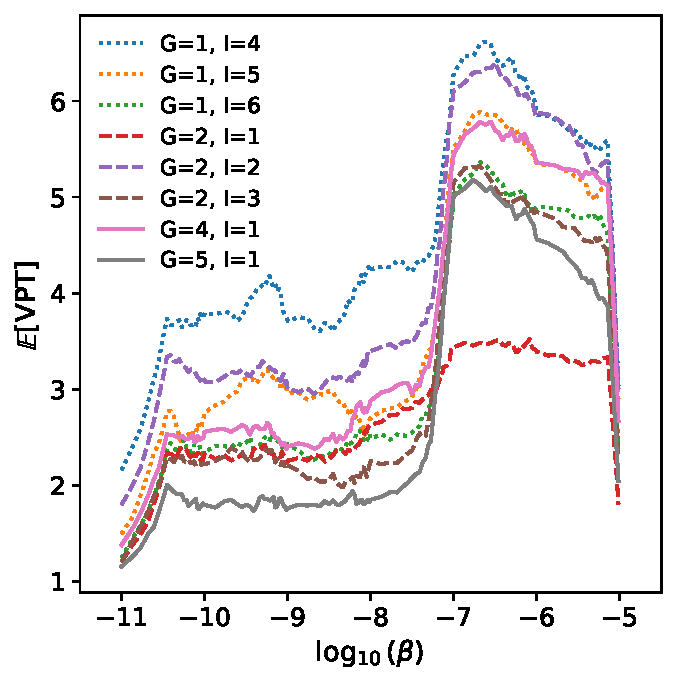
\includegraphics[scale=0.55]{plots/L96-localization-schemes.pdf}
    \caption{Estimates of mean VPT for different values of $\beta$ for different localization schemes for L96. The data shown here were generated using LocalSkip models with $D_r=4096$.}
    \label{fig:L96-loc}
\end{figure}

\begin{figure}[!htp]
    \centering
    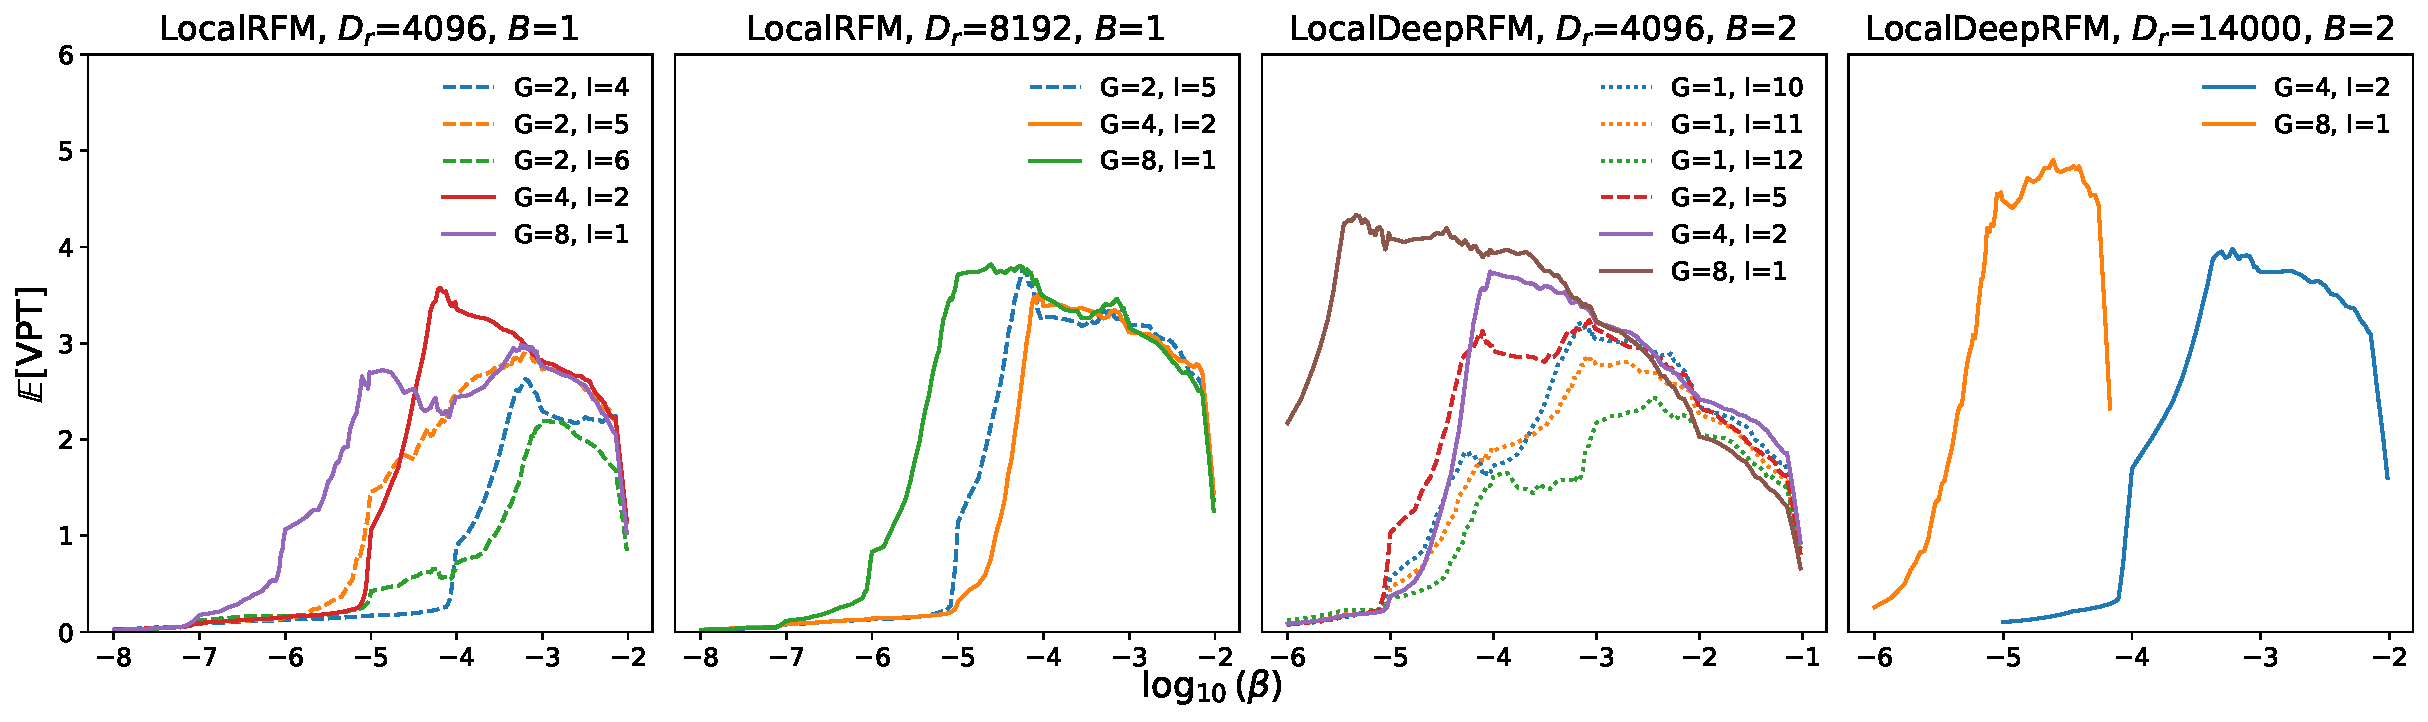
\includegraphics[scale=0.4]{plots/KS-200-localization-schemes.pdf}
    \caption{Estimates of mean VPT for different values of $\beta$ for different localization schemes for KS.}
    \label{fig:KS-loc}
\end{figure}

While choosing a localization scheme practitioners should consider several things such as hardware e.g. available GPU memory, model size, $D_r$, amount of training data $N$, inferences drawn from the covariance matrix or autocorrelation of the data, physical intuitions about the underlying dynamical system etc. If $G_2>G_1$ then for the same architecture and $D_r$, the model using scheme $(G_2, I_2)$ will typically have larger size compared to the model using scheme $(G_1, I_1)$. Since the GPU memory used during training is primarily a function of  $ND_r$,  for the same $N$ both models occupy roughly the same amount of memory on the GPU during training, despite the model using scheme $(G_1, I_1)$ having smaller size. Therefore, if our goal is to fit the largest possible model on the GPU during training, we should opt for the localization scheme with larger $G$. These considerations lead us to choose $(G, I)=(2, 2)$ for L96 and $(G, I)=(8, 1)$ for KS. These choices are consistent with \cite{platt2022systematic, vlachas2020backpropagation}.
